\section{Ergo state}
\label{sec:utxo}

\dnote{rewrite and provide detailed description of Ergo Box, AVL+ trees, digest nodes}
\dnote{it might be useful to add info about block structure~(Header+Block transactions+Extension+ADProofs), transaction structure}

To check a new transaction, a cryptocurrency client is not using the ledger (all the transactions happened before this
one). Instead, it is using the ledger state snapshot got from history. In Bitcoin Core reference implementation,
this snapshot is about active one-time coins, and a transaction is destroying some coins and also creating new ones.
In Ethereum, the snapshot is about long-living accounts, a transaction then is modifying monetary balance and internal memory of some accounts. Also, the
representation of the snapshot in Ethereum~(unlike Bitcoin) is fixed by the protocol, as authenticating digest of the
snapshot is written into a block header.

Ergo is representing the snapshot in the form of one-time coins, like Bitcoin. The difference is, in addition to monetary
value and protecting script, an Ergo coin contains user-defined data, and we use term {\em box} instead of {\em coin}.
Ergo box is made of registers~(and nothing but registers), every box in the system consists of 10 registers $R_0,R_1,\ldots,R_9$.
From these registers, four are filled with mandatory values, while the rest can contain arbitrary data:


\begin{itemize}
    \item{\em $R_0$: monetary value. } Amount of Erg locked in this box.
    \item{\em $R_1$: guard script. } Serialized script, protecting this box.
    \item{\em $R_2$: tokens. } A box can carry multiple tokens. This register contains an array of
    $token\_identifier -> amount$ pairs locked in this box.
    \item{\em $R_3$: tx info. } Contains declared creation height~(that should not be bigger then height of a block, carrying this transaction),
    unique identifier of transaction which created the box and also an index of the box in the transaction.
    \item{\em $R_4-R_9$: additional data. } Contains arbitrary user-defined data.
\end{itemize}


Using one-time immutable objects is the easiest and safest solution for replay and reordering attacks.
Also, it is easier to process transactions in parallel when they are not modifying the state of objects they
are accessing.
Also, with one-time coins, it seems it is easier to build fully stateless clients~\cite{chepurnoy2018edrax},
however, research in this area is still in the initial stage.
A major criticism for one-time coins says that this model is not suitable for non-trivial applications,
but Ergo has overcome such problems, and we have many non-trivial prototype applications built on top of
the Ergo Platform~(see~\ref{sec:contractual}).

The Ergo protocol fixes the ledger snapshot representation in the form of boxes not destroyed by previous transactions.
In details, a miner should maintain a Merkle-tree like authenticated data structure built on top of UTXO set and include
short digest (just 33 bytes) corresponding to UTXO set after application of a block into a header of the block.
This authenticated data structure is built on top of AVL+ tree~\cite{reyzin2017improving} and like a regular hash tree,
allows generating proofs of existence and non-existence of particular elements in a tree.
Thus users maintaining the full tree are capable to generate proofs that their boxes were unspent, while small 33 bytes
digest allows verifying these proofs.
Also, it allows to generate proofs of the tree modifications, that is enough to calculate a new tree digest on the verifier side.
In Ergo miner is enforced to generate proofs for block modifications, and a hash of this proof is included into
a block header as well as the digest of the resulting state.
So, light nodes that only keeps a small tree digest are able to verify the full block --- that all spent boxes where
removed from the state, all created boxes were added to it and no more changes where made.

Our improvements to the design of authenticated dictionaries reduce proof size and speed
up verification by 1.4-2.5 times, making them better suited for the cryptocurrency application.
For example, our proofs sizes are for about 3 times smaller, than proofs of Merkle Patricia trie used in Ethereum
for the same purposes:

\dnote{find image sources and insert images of a better quality}

\begin{figure}[H]
    \centering
    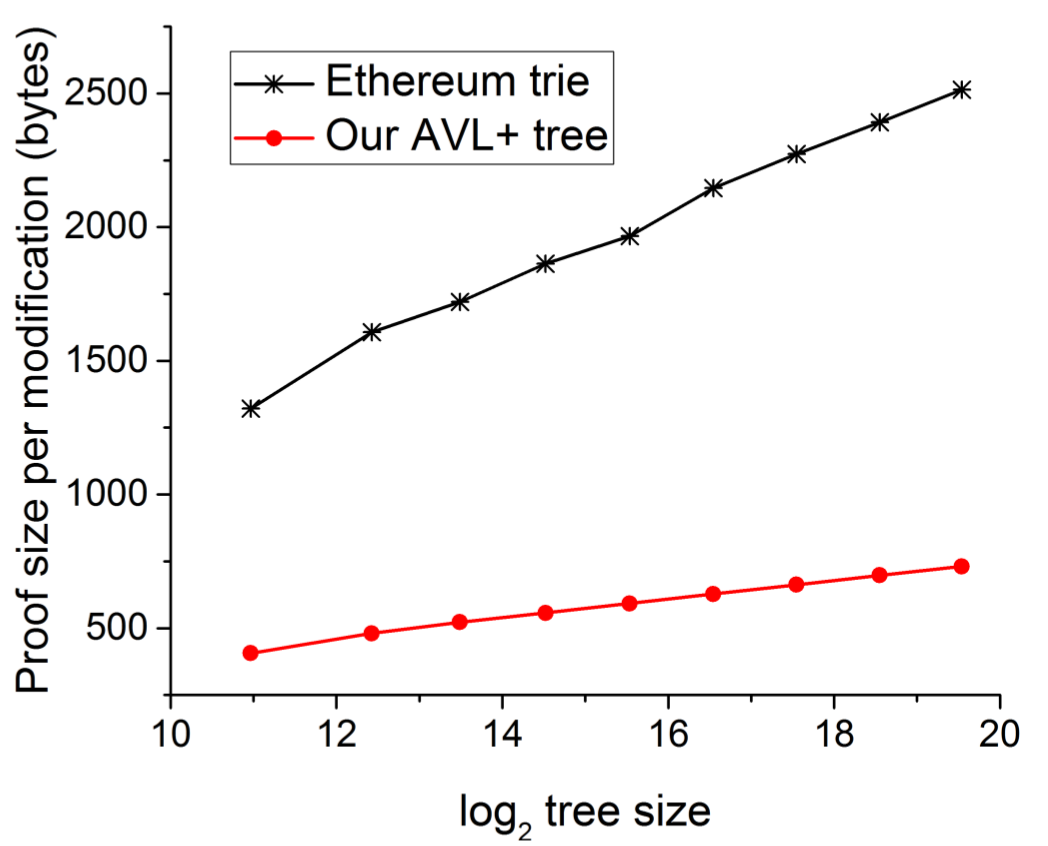
\includegraphics[width=0.5\textwidth]{img/proofSize.png}
    \caption{Proof size comparison with Merkle patricia trie
    \label{fig:proofSize} }
\end{figure}

Finally, proofs for multiple transactions in a single block are compressed together, reducing their total length
by approximately an additional factor of 2:

\begin{figure}[H]
    \centering
    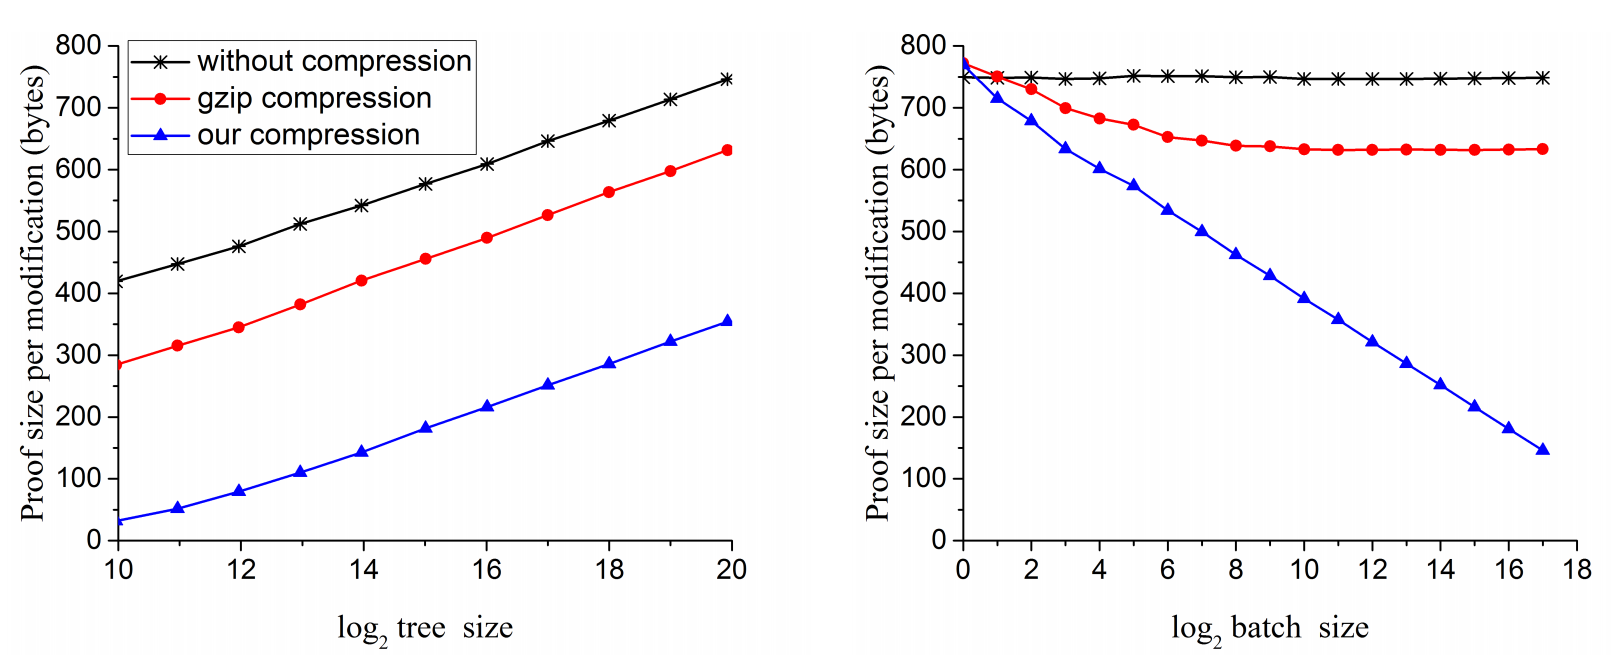
\includegraphics[width=\textwidth]{img/compression.png}
    \caption{Left: proof size per modification for 2000 transactions, as a function of starting tree size n.
    Right: proof size per modification for a tree with n = 1 000 000 keys, as a function of batch size B.
    In both cases, half of the modifications were inserts of new (key, value) pairs and half were changes
    of values for existing keys.
    \label{fig:compression} }
\end{figure}

Thus, Ergo state provide an efficient and secure way to prove existence or non-existence of certain elements in
it, as well as proofs for tree modifications.
These tree operations are supported by Ergo smart contract language, providing a way to implement complicated
contracts like discussed in~\ref{sec:contractual}





